\cotefile{78}
\scanpage{117}

on trouve

\[
\begin{aligned}
\Phi_{2p}(T)&=\Phi_p(-T)=T^{p-1}-T^{p-\unsure{2}}\ldots+1\\
\deleted{\unsure{\text{on a}}}\quad\Psi_{2p}(U)&=\Psi_p(-U)(-1)^{\frac{p-1}{2}}
\end{aligned}
\]

en car. $p$, les \deleted{solutions} \inserted{zéros de} \deleted{sont} $\Phi_{2p}(T)$ sont égales à $-1$, donc celles de $\Psi_{2p}$ sont égales à $-2$, qui est bien l'invariant du pol. régulier à $2p$ côtés. Donc en \uline{tte car.} $\ne 2$, la condition \unsure{nec.|n.} et \unsure{suffisante} pour qu'\deleted{\unsure{on ait}} l'inv. $\alpha$ définisse un pol. régulier à $2p$ côtés est\unsure{.|:} $\unsure{\Psi|\Phi}_{2p}(\alpha)=0$.

L'anneau modulaire est donc

\[
k'_{2p}=\mathbb Z[\tfrac12][U]/\Psi_{2p}(U).
\]

Reste enfin le cas $n=4$ ($=2.p$ avec $p=2$). Ici $\Phi_4(T)=T^2+1$, $\Psi_4(U)=\underset{\inserted{=F_4(U)}}{U}$, En car. 2, le\deleted{\unsure{s}} \inserted{seul} zéro de $\Psi_4$ est $0=-2$, donc qui définit bien le carré en car. 2. Donc ici

\[
{\unsure{k|K}}'_4=\mathbb Z[U]/U\simeq\mathbb Z
\]

i.e. il existe (à un isom unique près) une réalisation géom régulière de $\Pi_4$ et une seule sur un anneau $k$ donné, et celle-ci est \deleted{\unsure{eq}} fidèle quand l'anneau est un corps \ldots

% archive sheet number: 116

\scanpage{118}

\uline{Proposition} \unsure{Soient|Soit} $p$ nb premier, $r\geq 0$ un entier, $n'\geq 1$ avec $(p,n')=1$, $n=p^rn'$. Alors on a

\[
\Phi_n(T)\equiv\Phi_{n'}(T)^{\varphi(p^r)}\qquad\bmod p
\]

Récurrence sur $r+n'\geq1$. Si $r+n'=1$ i.e. $r=0$, $n'=1$, c'est trivial (NB $\varphi(1)=1$). Si $r+n'\geq2$, On aura pour tout diviseur $\delta\geq1$ de $n=p^rn'$, donc $\delta=p^sd$ ($0\leq s\leq r,\ 1\leq d\mid n'$) si $\delta\ne n$ i.e $(s\unsure{,|+}d)\ne(r,n')$ i.e. $s+d<r+n'$, par hyp de récurrence

\[
\Phi_\delta(T)=\Phi_{p^sd}(T)\equiv\Phi_d(T)^{\varphi(p^s)}\tag*{(1)}
\]

tandis que pour $\delta=n$ on \deleted{\unsure{écrira}}

\[
\inserted{\left[\Phi_{n'}(T)^{\varphi(p^r)}\right]}\,\Phi_n(T)=\Phi_{p^rn'}(T)\equiv\inserted{[\Phi_n(T)]}\,\Phi_{n'}(T)^{\varphi(p^r)}\deleted{\lambda(T)}\tag*{(2)}
\]

où

\[
\deleted{\lambda(T)=\frac{\Phi_n(T)}{\Phi_{n'}(T)^{\varphi(p^r)}}}
\]

Multipliant les relations (1) entre elles et avec (2), on trouve

\[
\Phi_{n'}(T)^{\varphi(p^r)}
\underbrace{\prod_{\delta\mid n}\Phi_\delta(T)}_{(T^n-1)}
\equiv\underbrace{\left(\prod_{\substack{0\leq\underline{s}\leq r\\1\leq\underline{d}\mid n'}}\Phi_d(T)^{\varphi(p^s)}\right)}_{
\displaystyle\prod_{0\leq\underline{s}\leq r}\underbrace{\left(\prod_{1\leq\underline{d}\mid n'}\Phi_d(T)\right)^{\varphi(p^{\unsure{s|d}})}}_{(T^{n'}-1)^{\varphi(p^s)}}}\Phi_n(T)
\]

% archive sheet number: 117

\scanpage{119}

d'où

\[
\Phi_{n'}(T)^{\varphi(p^r)}(T^n-1)\equiv\deleted{\unsure{\prod}}\,(T^{n'}-1)^{\sum_{s=0}^r\varphi(p^s)}\Phi_n(T)
\]

et comme $\sum_{s=0}^r\varphi(p^s)=1+(p-1)+(p^2-p)+\ldots+(p^r-p^{\unsure{r-1}})$ $=p^r$, on trouve

\[
\Phi_{n'}(T)^{\varphi(p^r)}(T^n-1)\equiv(T^{n'}-1)^{p^r}\Phi_n(T)
\]

Or

\[
T^n-1=(T^{n'})^{p^r}-(1)^{p^r}\equiv(T^{n'}-1)^{p^r}
\]

\deleted{\unsure{comme}} Donc divisant par $(T^{n'}-1)^{p^r}$, on trouve

\[
\Phi_n(T)^{\varphi(p^r)}=\Phi_n(T)
\]

\hfill cqfd.

\uline{Corollaire} Soient $k$ un corps de car. $p>0$, $n$ un entier \deleted{$\geq3,$} $\geq1$, $\alpha\in k$ une racine du polynôme semi-cyclotomique $\Psi_n$, i.e.

\[
\Psi_n(\alpha)=0
\]

Soit \deleted{$r\geq0$ tel que} \inserted{$p^r$ ($r\geq0$) la} plus grande puissance de $p$ qui divise $n$, donc

\[
n=p^rn',\qquad(p,n')=1.
\]

Alors le polygône régulier d'invariant $\alpha$ est d'ordre égal à $n'$ si $n'\geq3$, i.e.

% archive sheet number: 118

\scanpage{120}

\[
\left|\begin{aligned}
&n'\ne1,2,\quad\text{d'ordre }2p\text{ si }n'=2\quad(\text{donc }p\ne2\text{ !})\\
&\text{d'ordre }p\text{ si }n'=1.
\end{aligned}\right.
\]

\uline{Dém}. Posons en effet $\alpha=\unsure{\zeta|\int|\xi}+\zeta^{-1}$, où $\zeta$ appartient à un surcorps de $k$. La relation $\Psi_n(\alpha)=0$ signifie $\Phi_n(\zeta)=0$, et équivaut aussi, grâce à la proposition, à $\Phi_{n'}(\zeta)=0$, \deleted{Si $n'\geq3$,} \inserted{i.e. $\zeta$ est} \deleted{Celà signifie que $\Psi_{n'}(\alpha)=0$ donc que} \inserted{une racine de 1 d'ordre $n'$. Si} $n'\geq3$, celà signifie que l'ordre du polygône géométrique régulier d'invariant $\alpha$ est égal à $n'$, Si $n'=2$, que son ordre est $2p$, si $n'=1$ que son ordre est $p$, \hfill cqfd.

% archive sheet number: 119

\scanpage{121}

\deleted{$\varphi$} Si $n=\prod p_i^{r_i}$ \quad $\varphi(n)=\prod(p_i^{r_i}-p_i^{r_i-1})$

$\varphi(p^r)\geq6$ sauf si

\diagram{$\begin{array}{rc|c|c||c||c}
p^r=&2&4&8&3&5\\\cline{2-6}
\varphi(p^r)=&1&2&4&2&4
\end{array}$}

\[
\left.\begin{array}{ll}
\text{Cas }\varphi(n)=1&n=1,2\\
\multicolumn{2}{l}{[\text{Si }n\geq3,\ \varphi(n)\text{ est \uline{pair}}]}\\
\text{Cas }\varphi(n)=2&n=4,3,6
\end{array}\right\}\ \text{cas }\alpha\text{ entiers}
\]

\[
\text{Cas }\varphi(n)=4\quad\left\{\begin{array}{lll}
n=p^r&p=8,\ p=5&\\
n=p^rq^s&2.5=10&4.3=12
\end{array}\right\}\ \begin{gathered}\text{cas }\alpha\\\text{quadratiques}\end{gathered}
\]

\diagram{$\begin{array}{c|c|c|c||c|c||l}
n&1&2&4&3&6&\\\hline
\alpha&2&-2&0&-1&+1&
\end{array}$}

\diagram{$\begin{array}{c|c||c||c|c||}
n&8&12&5&10\\\hline
\alpha&\pm\sqrt 2&\pm\sqrt 3&\frac{-1\pm\sqrt5}{2}&\frac{1\pm\sqrt5}{2}\\
&\unsure{\{}\,\alpha^2-2=0&\alpha^2-3=0&\alpha^2+\alpha-1=0&\alpha^2-\alpha-1=0
\end{array}$}

Cas $\alpha$ cubiques \qquad $\varphi(n)=6$

\[
\begin{aligned}
n&=p^r&\varphi(n)&=p^r-p^{r-1}=6\\
n&=p^rq^s& &\bigl\{\,p^r=2,\ q^s=9,7
\end{aligned}
\]

\margin{On doit avoir $p\ne2$ (car $2^r-2^{r-1}=2^{r-1}$) \deleted{\unsure{et si}} Si $r=1\Rightarrow p=7$ Si $r\geq2$, $p\mid6$ donc $p=3$, on trouve $r=2$}

\diagram{$\begin{array}{c|c|c|}
n&9\quad\unsure{1|/}&7\\\hline
\alpha&\alpha^3-3\alpha+1=0&
\tikz[baseline=(e.base)]{\node[inner sep=0pt] (e) {$\alpha^3-2\alpha+\alpha^2-1=0$};\draw[thin] (-.53,-.12) .. controls (-.12,-.47) and (-.10,.45) .. (.21,.16);}\rlap{\tikz[remember picture,overlay]\coordinate (cubicseven);}\\\hline
\end{array}$}

(exemples d'équations du $3^{\mathrm e}$ degré non résolubles par radicaux carrés) \ldots

\diagram{$\begin{array}{c|c|c|}
\tikz[remember picture,overlay]{\coordinate (cubiceighteen);\draw[thin] (cubicseven) .. controls +(right:5mm) and +(left:7mm) .. (cubiceighteen);}n&18&14\\\hline
\alpha&\alpha^3-3\alpha-1=0&\alpha^3-\alpha^2-2\alpha+1=0
\end{array}$}

\figure{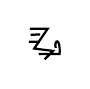
\begin{tikzpicture}[x=0.38cm,y=0.38cm]
\draw[line width=.8pt] (0,.88)--(.59,.88)--(.14,.22)--(.77,.14)--(.49,-.14) (.02,.68)--(.34,.69) (-.04,.45)--(.33,.45) (.29,.04)--(.99,.04).. controls (1.02,.65) and (.79,.48) .. (.86,.24);
\end{tikzpicture}}

% archive sheet number: 120

\scanpage{122}

\[
\begin{aligned}
&\unsure{u}\quad\deleted{u(\unsure{e_1})}\\
&\deleted{\check u(\unsure{u'|x'} )\otimes{}}\qquad\deleted{{}^{t}u}\\
\deleted{u}\quad&\deleted{u(\unsure{x})\otimes x}\qquad({}^{t}u\,x')\otimes x=x'\otimes ux
\end{aligned}
\]

\figure{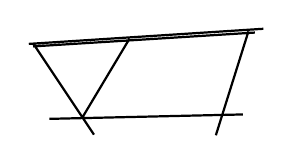
\begin{tikzpicture}[x=.9cm,y=.8cm]
\draw[thick] (-.06,1.22)--(3.25,1.46) (0,1.18)--(3.13,1.40) (0,1.23)--(.86,-.22) (.23,.03)--(2.96,.1) (.69,.04)--(1.36,1.3) (2.58,-.23)--(3.04,1.42);
\end{tikzpicture}}

\[
\deleted{\bigl[{}^tu(-2e'_1+e'_2)\bigr]\otimes e_1=(-2e'_1+e'_2)\otimes ue_1}
\]

\figure{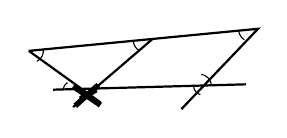
\begin{tikzpicture}[x=.91cm,y=.85cm]
\draw[thick] (0,1.1)--(3.2,1.43)--(2.13,.23) (0,1.1)--(1,.33) (.34,.52)--(3.03,.6) (.62,.26)--(1.73,1.28);
\draw (0.2,1.13) arc(12:-62:.17) (1.46,1.25) arc(180:237:.17) (2.93,1.40) arc(185:236:.18) (2.55,.59) arc(5:78:.18) (2.3,.57) arc(183:251:.14) (.48,.53) arc(174:122:.13);
\draw[line width=2pt] (.65,.28)--(.97,.59) (.62,.57)--(1,.29) (.72,.38)--(.94,.52);
\end{tikzpicture}}

\[
\begin{aligned}
\deleted{{}^tu(e'_1)=\sum u_{1i}e'_i}&&\deleted{ue_{\unsure{i|1}}=\sum_i u_{i1}e_i}\\
\deleted{{}^tu\,e'_2=\sum u_{2i}e'_i}
\end{aligned}
\]

\[
\deleted{\sum_i(-2u_{1i}+u_{2i})e'_i\otimes e_1} \deleted{{}=\sum(-2u_{i1})e'_1\otimes e_i+\sum u_{i1}e'_2\otimes e_{\unsure{i}}}
\]

\[
\deleted{\unsure{\sum-2}u_{1i}\ \cdots\;-\;-\; -}\qquad
\deleted{\unsure{+}u_{i\unsure{2|1}}=}
\]

\diagram{$\deleted{\begin{array}{cccc}
e'_1\otimes e_1&e'_2\otimes e_1&\cdots&e'_n\otimes e_1\\\cline{1-2}
e'_1\otimes e_2&e'_2\otimes e_2&&\\
\vdots&\vdots&&\\
e'_1\otimes e_n&e'_2\otimes e_n&&
\end{array}}$}

% margin note written sideways

\margin{$\unsure{F\subset|F<}\qquad x+\langle x,x'\rangle x\qquad-x$ \quad $\unsure{x'|x?}\quada+\langle a,a'\rangle x$}

\[
\deleted{\left\{\begin{aligned}u_{i1}&=0\\-2u_{i1}&=0\end{aligned}\right.\qquad i\geq2}
\]

\[
\begin{aligned}
\deleted{\left\{\vphantom{\Large A}u_{2i}=2u_{1i}\right.\quad i\geq3}
&\qquad\deleted{-2u_{11}+u_{21}=-2u_{11}}\\
&\qquad\deleted{-2u_{12}+u_{22}=u_{11}}
\end{aligned}
\]

\margin{i.e. $u_{21}=0$ déjà \uline{connu}}

\diagram{$\deleted{\begin{array}{ccccc|}
\lambda&u_{12}&u_{13}&\cdots&u_{1n}\\
0&\unsure{\lambda+2u_{12}|\lambda}&2u_{13}&\cdots&2u_{1n}\\
\vdots&\multicolumn{4}{c|}{\raisebox{-.45em}{\tikz{\draw (0,0) ellipse (1.5cm and .32cm);}}}\\
0&&&&
\end{array}}$}

\[
\unsure{\downarrow}\qquad\unsure{'}
\]

% margin note written upside down

\margin{$\unsure{\check E}\otimes\check E^{\unsure{\lambda}}$}

% margin note written upside down

\margin{$\deleted{\lambda=1}\quad\lambda(T-1)^{\unsure{\nu}-1}(T+1)$ \quad $(\lambda-1)^{\nu-1}(\lambda+1)=0$}

% margin note written upside down

\margin{$1\qquad x'_i\quad\dfrac{z'_i}{x'_i}$}

% margin note written upside down

\margin{$z'\otimes z=u'\otimes u+(1-\lambda)\,\mathrm{id}$}

% archive sheet number: 121

\scanpage{123}

$\Phi_n(T)$ polynôme minimal sur $\unsure{\mathbb Q|Q}$ d'une racine primitive $n$-ième $\zeta$ de 1

\margin{$n\in\mathbb N^*$}

$F_n(T)$ polynôme minimal de $\zeta+\zeta^{-1}$

Si $n\ne1,2$, on a $\Phi_n(T)=T^{\varphi'(n)}F_n(T+T^{-1})$ \quad $(\varphi'(n)=\varphi(n)/2)$

\margin{$\Phi_n,F_n\in\mathbb Z[T]$ pol. unitaires}

\[
\begin{aligned}
\deg\Phi_n&=\varphi(n)\quad\text{(indicateur d'Euler, }=\operatorname{card}(\mathbb Z/n\mathbb Z)^*\text{)}\\
\deg F_n&=\begin{cases}1&\text{si }n=1,2\quad(F_1(T)=T-2,\ F_2(T)=T+2)\\
\varphi(n)/2&\text{si }n\geq3\end{cases}
\end{aligned}
\]

\[
\prod_{\substack{d\in\mathbb N^*\\d\mid n}}\Phi_n(T)=T^n-1
\]

donne mode de calcul par récurrence \unsure{multiplicative} sur $n$.

\diagram{$\left\{\begin{array}{l}
F_1(\deleted{T}U)=\deleted{T}U-2\\
F_2(\deleted{T}U)=\deleted{T}U+2\\
F_3(\deleted{T}U)=\deleted{T}U+1\\
F_4(\deleted{T}U)=\deleted{T}U\deleted{\unsure{{}^2-2}}\\
F_5(\deleted{T}U)=\deleted{T}U^2+\deleted{T}U-1\\
F_6(\deleted{T}U)=\deleted{T}U-1\\
F_7(\deleted{T}U)=\deleted{T}U^3+\deleted{T}U^2-2\deleted{T}U-1\\
F_8(\deleted{T}U)=\deleted{T}U^2-2\\
F_9(\deleted{T}U)=\deleted{T}U^3-3\deleted{T}U+1\\
F_{10}(\deleted{T}U)=\deleted{T}U^2-\deleted{T}U-1\\
\ldots
\end{array}\right.\quad
\left\{\begin{array}{l}
\Phi_1(T)=T-1\\
\Phi_2(T)=T+1\\
\Phi_3(T)=T^2+T+1\\
\Phi_4(T)=T^2+1\\
\Phi_5(T)=T^4+T^3+T^2+T+1\\
\Phi_6(T)=T^2-T+1\\
\Phi_7(T)=T^6+T^5+T^4+T^3+T^{\unsure{1|2}}+T^{\unsure{2|1|{}}}+1\\
\Phi_8(T)=T^4+1\\
\Phi_9(T)=T^6+T^3+1\\
\Phi_{10}(T)=T^4-T^3+T^2-T+1\\
\ldots
\end{array}\right.$}

(donner aussi les cas $n=12,14,18\ldots$)

\[
\left\{\begin{aligned}
&\Phi_p(T)=1+T+\ldots+T^{p-1}\\
&\text{si }p\text{ premier}\\
&F_p(T)=S_0(T)+S_1(T)+\ldots+S_{p'}(T)
\end{aligned}\right.
\]

où $p=2p'+1$ i.e. $p-1=2p'$ ($p$ \unsure{nb|est} premier impair), et les

\[
S_{\unsure{n|p}}(\deleted{T}U)\in\mathbb Z[\deleted{T}U]\qquad(n\in\mathbb N^*)
\]

sont caractérisés par

\[
\left\{\begin{aligned}
&S_0(\deleted{T}U)=1\\
&T^n+T^{-n}=S_n\unsure{'}(T+T^{-1})\qquad n\geq1
\end{aligned}\right.
\]

donc

\[
\left\{\begin{aligned}
S_0(\deleted{T}U)&=1\\
S_1(\deleted{T}U)&=\deleted{T}U\\
S_2(\deleted{T}U)&=\deleted{T}U^2-2\\
S_3(\deleted{T}U)&=U^3-3U\\
&\ldots
\end{aligned}\right.
\]

Calcul récurrent des $S_i$ par formule

\[
\deleted{\unsure{S_n(T|S_n(T)}}\quad U^n=\sum_{0\leq i\leq[\frac n2]}\binom ni S_{n-2i}(U)\qquad n\geq1
\]

d'où

\[
S_n(U)=U^n-\sum_{1\leq i\leq[\frac n2]}\binom ni S_{n-2i}(U)
\]

% archive sheet number: 122

\scanpage{124}

\[
\left\{\begin{aligned}
\deleted{F}\Phi_{2p}(T)&\inserted{=F_p(-T)\deleted{\unsure{(-1)^{\varphi'(p)}}}}
=1-T+T^2+\ldots+(-1)^{p-1}T^{p-1}\qquad\text{$p$ nb premier impair}\\
\deleted{\Phi}F_{2p}(T)&=\inserted{(-1)^{p'}}\Phi_p(-T)
=\bigl(S_0(T)-S_1(T)+\ldots+(-1)^{p'}S_{p'}(T)\bigr)(-1)^{p'}
\end{aligned}\right.
\]

\begin{center}\rule{1cm}{.4pt}\end{center}

Sur un corps \inserted{$k$ alg clos de} car. quelconque $p$, les racines de $F_n(T)$ sont les racines \uline{primitives} \deleted{\unsure{$n$-ièmes}} \inserted{\deleted{i.e.} $n'$-ièmes} de 1, chacune avec leur multiplicité, qui est

\[
\left\{\begin{aligned}
&\text{multiplicité }1\quad\text{si }(p,n)=1\\
&\text{multiplicité }\varphi(p^r)\quad\text{si }n=p^rn',\quad(n,n')=1,\quad r\in\mathbb N
\end{aligned}\right.
\]

Si $(\zeta_i)\deleted{\unsure{_{1\leq i}}}$ sont les racines \inserted{primitives \deleted{\unsure{distinctes $n'$ de 1|distinctes $n$-ièmes}}} \deleted{\unsure{deux à deux}} $n'$ièmes de 1, on a donc

\[
\Phi_n(T)=\left(\prod(T-\zeta_i)\right)^{\varphi(p^r)}=\Phi_{n'}(T)^{\varphi(p^r)}\quad\text{dans }k[T]
\]

\deleted{\unsure{(il vient donc pour $k$ corps de car. $p$}} on a

\[
\Phi_n(T)=\Phi_{n'}(T)^{\varphi(p^r)}\quad\text{dans }\unsure{\Phi_p(T)|\mathbb F_p(T)}
\]

i.e

\[
\Phi_n\equiv\Phi_{n'}^{\varphi(p^r)}\quad\bmod p
\]

En particulier

\[
\left\{\begin{aligned}
\Phi_{p^r}(T)&\equiv(T-1)^{\varphi(p^r)}\quad\bmod p\\
\Phi_p(T)&\equiv(T-1)^{p-1}\quad\bmod p\qquad -
\end{aligned}\right.
\]

\deleted{\unsure{Les}} Les racines de $F_n(T)$ \deleted{\unsure{dans}} $k$ sont les \unsure{éléments|élémts} de la forme $\zeta+\zeta^{-1}$ ($\zeta$ racine primitive $n'$-ième de 1), chacun avec la multiplicité $\varphi(p^r)\deleted{\unsure{/2}}$ -- \deleted{\unsure{donc}} \inserted{sauf si} $n'=1$ ou 2, où la multiplicité est $\varphi(p^r)/2$.

\[
\left\{\begin{aligned}
F_n(T)&\equiv F_{n'}(T)^{\varphi(p^r)}\quad\bmod p\qquad\text{si }n'\ne1,2\\
F_n(T)&\equiv F_{n'}(T)^{\varphi(p^r)/2}\quad\bmod p\qquad\text{si }n'=1\text{ ou }2
\end{aligned}\right.
\]

en particulier

\[
\left\{\begin{aligned}
F_{p^r}(T)&\equiv\deleted{\unsure{F_p(T)^{\varphi(p)}}}\,(T-2)^{\varphi(p^r)}\quad(p)\\
F_p(T)&\equiv(T-2)
\end{aligned}\right.
\]

% archive sheet number: 123

\scanpage{125}

Multiplicité \inserted{$\mu$} des racines \unsure{de|des} $F_n$ \inserted{($n\geq3$)} dans $k$ de car $p>0$,

\[
n=n'p^r\qquad((n,n')=1,\ r\in\mathbb N)
\]

1) $n'\ne1,2$ (donc $F_{n'}(T)$ de degré $\varphi(n')/2$) : $\mu=\varphi(p^r)$, donc

\[
F_n(T)\equiv F_{n'}(T)^{\varphi(p^r)}\quad\bmod p
\]

2) $n'=1$ ou 2 (donc $F_{n'}(T)$ de degré $1=\varphi(n')$) \deleted{et $\unsure{p^r\ne2|p^r\ne1,2}$} et $p^r\ne2$ i.e. $n\ne4$ -- donc \deleted{$\unsure{p^r\ne2|\varphi(p^r)}$} \inserted{$F_{p^r}(T)$} de degré $\varphi(p^r)/2$

\margin{$\mu=\varphi(p^r)/2$}

\[
F_n(T)\equiv F_{n'}(T)^{\varphi(p^r)/2}\ \bmod(p)\quad
\left\{\begin{aligned}
&(T-2)^{\varphi(p^r)/2}\quad\text{si }n=p^r\\
&(T+2)^{\varphi(p^r)/2}\quad\text{si }n=2p^r
\end{aligned}\right.
\]

\deleted{3) $n=4=p^2$, $p=2$ \quad $F_4(T)\equiv(T-2)^2\ \bmod 2\equiv(T^{\unsure{2|{}}}+2)^{2}\equiv T^{\unsure{2}}\ \bmod2$}

\deleted{$\unsure{\Vert}\quad F_{n'=1}(T)^{\unsure{\varphi(p^r=4)|\varphi(4)=4}}$ (comme cas 1)}

En particulier, si $p$ premier $\ne2$, on a

\[
\begin{aligned}
F_p(T)&\equiv(T-1)^{p'}\quad\bmod p\\
F_{2p}(T)&=(T+1)^{p'}\quad\bmod p
\end{aligned}
\]

\margin{$p'=(p-1)/2$ \quad\deleted{\unsure{($p$ pr}}}

% archive sheet number: 124

\scanpage{126}

\[
\left.\begin{aligned}
\alpha\in B_{\unsure{n(p)|p}}&=\mathbb Z[\deleted{T}U]/\deleted{\unsure{\Phi}}F_p(U)\\
\zeta\in A_p&=\mathbb Z[T]/\Phi_p(T)
\end{aligned}\right|\quad\text{normaux}\qquad p\text{ premier impair}
\]

ils sont étales sur $\mathbb Z$ en les \deleted{$\unsure{p}$} $\ell\in\operatorname{Spec}(\mathbb Z)$, $\ell\ne p$ car en ces pts les racines de $F_p,\Phi_p$ sont distinctes.

Ramifiés en $\ell=p$ (une seule racine en \unsure{corps|carps} de car $p$)

\[
(\zeta-1)^{p-1}\equiv0\quad(p)\qquad\text{dans }A_{\deleted{\unsure{(p)}}}=A_{(p)}
\]

\[
\deleted{\unsure{1+T+\cdots}}\quad\zeta^{p-1}-(p-1)\zeta^{p-2}+\frac{(p-1)(p-2)}2\zeta^{p-3}-\ldots\ \deleted{\unsure{p}}\ 1
\]

\[
\deleted{1+T+\ldots+T^{p-1}\equiv(T-1)^{p-1}\quad(p)}
\]

\[
\begin{aligned}
(\zeta-1)^{p-1}&=(\zeta-1)^{p-1}-F_p(\zeta)\\
&=p\zeta^{p-2}+\left(\frac{(p-1)(p-2)}2-1\right)\zeta^{p-\deleted{2}\inserted{3}}+
\left(-\frac{(p-1)(p-2)(p-3)}6-1\right)\zeta^{p-4}\ldots
\end{aligned}
\]

\figure{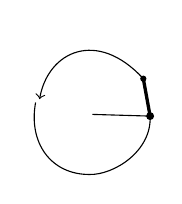
\begin{tikzpicture}[x=.72cm,y=.72cm]
\draw (1.02,0).. controls (1.05,-.62) and (.38,-1.04) ..(-.05,-1.03).. controls (-.74,-1.03) and (-1.13,-.46) ..(-1,.24);
\draw[->] (.90,.66).. controls (.08,1.55) and (-.78,1.14)..(-.93,.30);
\draw (0,.03)--(1.02,0);\draw[very thick] (1.02,0)--(.90,.66);\fill (1.02,0) circle (.07) (.90,.66) circle (.055);
\end{tikzpicture}}

\[
\frac1p(\zeta-1)^{p-1}=\zeta^{p-2}+
\]

\[
\begin{aligned}
N\left(\frac1p(\zeta-1)^{p-1}\right)&=\frac1{p^{p-1}}N(\zeta-1)^{p-1}.\\
N(\zeta-1)&=\prod_1^{p-1}(\zeta_i-1)=\deleted{\unsure{\prod|\varepsilon}}\cdot\prod(1-\zeta_i)=F_p(1)=\underbrace{1\ldots+1}=p\\
N\left(\frac1p(\zeta-1)^{p-1}\right)&=1
\end{aligned}
\]

\[
\boxed{(\zeta-1)^{p-1}=pu}\qquad u\ \text{\uline{unité}}
\]

Donc $(\zeta-1)A\supset pA$ \deleted{$\unsure{(\zeta-1|(\zeta-1)}$} donc

\[
\begin{aligned}
A/(\zeta-1)A&=(\underbrace{A/pA}_{A_0})/(\zeta-1)A_0=\bigl(\mathbb F_p[T]/(T-1)^{p-1}\bigr)/(T-1)\\
&=\mathrm F_p
\end{aligned}
\]

Donc $(\zeta-1)A$ est un idéal \uline{maximal}

% archive sheet number: 125

\scanpage{127}

$F_{p^r}$ \qquad $\varphi'=\left\{\vphantom{\dfrac12}\right.\varphi(p^r)/2$ si $p^r\ne2$

\[
\begin{aligned}
(\alpha-2)^{\varphi'}&=pu\\
N(\alpha-2)^{\varphi'}&=p^{\varphi'}N(u)\\
N(\alpha-2)&=\prod(\alpha_i-2)=(-1)^{\varphi'}\prod\overbrace{(2-\alpha_i)}^{(\zeta'_i-1)(\zeta''_i-1)}
=(-1)^{\varphi'}\underbrace{F_{p^r}(2)}_{p}=(-1)^{\varphi'}\Phi_{p^r}(1)\\
&\hspace{23em}=(-1)^{\varphi'}
\end{aligned}
\]

$8+4-4-1$

\deleted{$A_p B$} $A_{p^r},B_{p^r}$ sont anneaux de Dedekind

\[
A_{n'p^r}
\]

\[
(\zeta-1)^{\unsure{\cdot|'}}
\]

\[
\begin{aligned}
\mathbb F_p[T]/\Phi_n(T)&=\mathbb F_p[T]/\deleted{\unsure{(T-1)^{\varphi(p^r)}}}\,\Phi_{n'}(T)^{\varphi(\unsure{p^r})}\\
&=\deleted{\unsure{\mathbb F_p[T]/\Phi_{n'}(T^{p^r})}}
\end{aligned}
\]

\[
\prod_{(r,n')=1}(T-\zeta^{r}_{\unsure{1}})\bigg/\prod(T-\zeta_i)^{\varphi(p^r)}
\]

\[
T\unsure{\cdot|-}1\qquad \unsure{T^n=|\deleted{T^n}}\quad1+T\ldots+T^{n'-1}
\]

$n'$ premier à $p$ \hfill $T^{p^r}-\zeta=0$ mais peut-être pas à $p-1$ \ldots !

\[
\begin{aligned}
T\quad\unsure{\zeta}&\qquad A_{n'}\subset A_n&&\zeta!\\
&\zeta'=\zeta^{p^r}\qquad\zeta-\zeta'&&{\zeta'}^{\unsure{(p^r)}}\\
&N_{A_n/A_{n'}}(\zeta-1)
\end{aligned}
\]

\diagram{\begin{tikzcd}[ampersand replacement=\&,column sep=small]
\underbrace{\mathrm F_p[T']/(\Phi_{\unsure{p'|n'}}(T'))}_{\substack{\text{$k_p$-alg des racines}\\\text{de l'équation cycl. }\Phi_{n'}.}}[T]\unsure{'} /(T^{p^r}-T')\arrow[r,"\unsure{\text{épi}|\text{cf.}}"]\& A_n\otimes\mathbb F_p
\end{tikzcd}}

\[
\deleted{\unsure{(\varphi(2))}}\qquad\deleted{\unsure{\Phi_{p^r}|\Phi_n}}\qquad\deleted{\unsure{T^{p^r}-(T')^{p^r}}}\qquad T^{\varphi(p^r)}+
\]

% archive sheet number: 126

\scanpage{128}

\[
\begin{aligned}
(\alpha-2)^{p'}&\equiv0\quad(p)\\
(\alpha-2)^{p'}&=pu\\
N(\alpha-2)^{p'}&=p^{p'}N(u)
\end{aligned}
\]

\[
\begin{aligned}
N(\alpha-2)&=\prod(\alpha_i-2)=(-1)^{p'}\prod
\underset{\substack{\deleted{\unsure{\zeta'_i+\zeta''_i|\zeta'_i\zeta''_i}}\\\deleted{\unsure{(1-\zeta'_i)(1-\zeta''_i)}}}}{\underbrace{\overset{(\zeta'_i-1)(\zeta''_i-1)}{(2-\alpha_i)}}}
=(-1)^{p'}F_p(2)=(-1)^{p'}\Phi_p(1)\\
&\hspace{22em}=(-1)^{\unsure{p'}}
\end{aligned}
\]

\[
\deleted{\alpha_i-2=\zeta_{i'}^2+\zeta_{i'}^{-2}-2=(\zeta_{i'}-\zeta_{i'}^{-1})^2}\ -
\]

\[
F_{\unsure{3|7|5}}\quad 8+4-4-1\qquad\boxed{F_p(2)=p}\ ?
\]

\[
\deleted{\unsure{B|A}=B[T]}\qquad
\begin{aligned}
(\zeta-1)(\zeta^{-1}-1)\\
=1+1-\alpha
\end{aligned}
\]

\diagram{\begin{tikzcd}[ampersand replacement=\&]
B[T]/(T^2-\alpha T+1)\arrow[r,"\text{iso?}"]\& A
\end{tikzcd}}

\begin{center}\rule{1.5cm}{.4pt}\end{center}

\[
\begin{aligned}
&\unsure{\zeta|2}\\
(\zeta-1)^\varphi&\equiv\deleted{\unsure{p}}\,\unsure{0}\quad(p)\\
(\deleted{\unsure{\xi}}\zeta-1)^\varphi&=pu\\
N(\deleted{\unsure{\xi}}\zeta-1)^\varphi&=p^\varphi N(u)
\end{aligned}
\]

\[
\prod(\zeta_i-1)=(-1)^\varphi\prod_i(1-\zeta_i)=(-1)^\varphi\underbrace{\deleted{\unsure{F}}\Phi_{p^r}(1)}_{\shortparallel\,p}
\]

\[
\left\{\prod_{\substack{d\mid p^r\\ d\ne1}}\Phi_n(T)=\deleted{T^n}\ 1+T\ldots+T^{\unsure{n-1|i-1|p^r-1}}=p^r\right.
\]

\[
\deleted{\prod_{d\mid p^r}p={}}\qquad\deleted{\Phi_p(1)\Phi_{p^2}(1)={}}\qquad\Phi_{p^r}(1)=p
\]

\[
p\quad p^2\ \ldots\ p^r
\]

% archive sheet number: 127

\scanpage{129}

\diagram{$\begin{array}{ccc}
&& (n',n'')=1\\
\zeta\in&A_{n'n''=n}&\supset A_{n''}\ni\zeta''\\
&\cup&\\
\zeta'\in&A_{n'}&
\end{array}\qquad
G=(\mathbb Z/n\mathbb Z)^*=
\underset{(\mathbb Z/n'\mathbb Z)^{\unsure{*}}}{\underset{\shortparallel}{G'}}
\times\underset{(\mathbb Z/n''\mathbb Z)^*}{\underset{\shortparallel}{G''}}$}

\diagram{\begin{tikzcd}[ampersand replacement=\&]
\underbrace{A_{n'}\underset{\mathbb Z}{\otimes}A_{n''}}_{\text{normal par hyp. de réc.}}\arrow[r,"\sim"]\&A_{n'n''}
\end{tikzcd}}

\[
\begin{aligned}
&B&&\zeta_i\eta_j+\zeta_i^{-1}\eta_j^{-1}\\
&\varphi(1)=1\\
&\varphi(2)=1
\end{aligned}
\]

\diagram{\begin{tikzcd}[ampersand replacement=\&]
B_n[T]/(T^2-\alpha T+1)\arrow[r]\& A_n
\end{tikzcd}}

\[
\left\{\begin{aligned}
\alpha_n&\longmapsto\zeta_n+\zeta_n^{-1}\\
T&\longmapsto\zeta_n
\end{aligned}\right.
\]

\[
\begin{aligned}
\mu_n&\supset\mu_n^*\deleted{\unsure{{}_n}}=\operatorname{Spec}\mathbb Z[T]/\Phi_n(T)\\
\mu_{n'}&\supset\mu_{nn'}^*=\mu_n^{\unsure{c|*}}\mu_{n'}\\
\mu_n^*/\{\pm1\}&=\deleted{\unsure{G}}\ \widetilde\mu_n^*
\end{aligned}
\]

\[
\begin{aligned}
B_n=A_n^{\unsure{\zeta|\sigma}}\qquad
\sigma(F+GT)&=F+G(U-T)\\
&=(F+GU)-GT\\
\sigma(F+GT)&=F\unsure{{}+G|\alpha}T\ \Longleftrightarrow\
\left\{\begin{array}{l}GU=0\qquad G=-G\\
\Longleftrightarrow\ \unsure{G|C}=0\end{array}\right.
\end{aligned}
\]

\diagram{\begin{tikzcd}[ampersand replacement=\&,column sep=small]
A=\mathbb Z[T,T^{-1}]\arrow[r]\&\mathbb Z[T]/\Phi_n(T)=A_n\arrow[d,leftrightarrow]\\
B=\mathbb Z[U]=\mathbb Z[T]^\sigma\arrow[u,phantom,"\unsure{\cup|\uparrow|\rotatebox{90}{$\hookrightarrow$}}" description]\arrow[r]\&\mathbb Z\unsure{(U]|[U]|(U)}/F_n(U)=B_n
\end{tikzcd}}

\diagram{\begin{tikzcd}[ampersand replacement=\&,column sep=small]
G_m\arrow[d]\&[-1em]\supset\mu_n\supset\mu_n^{\unsure{c|*}}\&\\
\mathbb E'\&\widetilde\mu_n/\pm1\arrow[l]\&\widetilde\mu_n^*\arrow[l]\\
\shortparallel\&\&\\
G_m/\sigma\&\&
\end{tikzcd}}

\[
\begin{aligned}
U&=T+T^{-1}& F_n(U)&=F_n(T+T^{-1})=T^{-\varphi'}\Phi_n(T)\\
\sigma(T)&=T^{-1}&&\underline{T}^{-1}=U-T
\end{aligned}
\]

\[
\deleted{\mathbb Z[T]/(T^n-1)}
\]

\uline{$n\ne1,2$}

\diagram{\begin{tikzcd}[ampersand replacement=\&]
A\& B[S]/(S^2-US+1)\arrow[l,"\sim"']\\
\&\shortparallel\\
\& B[\dot S]=B.1\oplus B.\dot S
\end{tikzcd}}

i.e. $A$ module libre sur $B$ de base $1,T$

\[
T^{2n}=T^n
\]

\[
\begin{aligned}
\deleted{F+T}\quad &F(U)+TG(U)=0& TG(U)&=T^{-1}G(U)\\
\Downarrow\quad &F(U)+T^{-1}G(U)=0&(T^2-1)G(U)&=0\qquad G(U)=0\quad\text{\unsure{puisque}}
\end{aligned}
\]

% archive sheet number: 128

\scanpage{130}

\diagram{\begin{tikzcd}[ampersand replacement=\&,column sep=small]
\unsure{B|A}\arrow[dr,dash]\&\& B'\arrow[dl,dash]\\
\&A\&
\end{tikzcd}}

\diagram{\begin{tikzcd}[ampersand replacement=\&,column sep=small]
\&\&X\times_S\!X\arrow[dl,dash]\arrow[dr,dash]\&\&\\
G\&X\arrow[dr,dash]\&\&X'\arrow[dl,dash]\&G'\\
\&\&s,s'\in S\&\&
\end{tikzcd}}

$X$ tot. ramifié en $s$, étale en dehors

$X'$ tot. ramifié en $s'$, étale en dehors

$X,X'$ normaux irréd.

$X\times_S X'$ est \unsure{norm.|normal|connexe} ?

\diagram{\begin{tikzcd}[ampersand replacement=\&,column sep=small]
\&\pi_1(S-\{s,s'\})\arrow[dl,dash]\arrow[dr]\&\\
\pi_1(S-s)\arrow[dr]\&\&\pi_1(S-s')\arrow[dl]\\
\&\pi_1(S)\&
\end{tikzcd}}

\diagram{\begin{tikzcd}[ampersand replacement=\&,column sep=small]
\&G*\mathbb Z*\mathbb Z\arrow[dl]\arrow[dr]\&\&G\times G'\\
X*\mathbb Z\arrow[dr]\&\&G*\mathbb Z\arrow[dl]\&\\
\&G\&\&
\end{tikzcd}}

\diagram{\begin{tikzcd}[ampersand replacement=\&,column sep=small]
\&\deleted{\unsure{X}}\arrow[dl,dash]\arrow[dr,dash]\&\\
\deleted{X_s}\arrow[dr]\&\&\deleted{X'_s}\arrow[dl]\\
\&S\&
\end{tikzcd}}

\figure{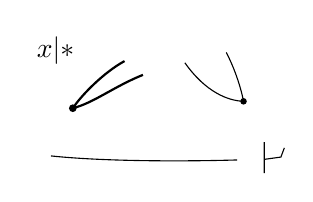
\begin{tikzpicture}[x=.73cm,y=.73cm]
\node at (-.2,1.20) {$\deleted{\unsure{x|\ast}}$};
\draw[thick] (1.00,1.02).. controls (.65,.83) and (.26,.44)..(.10,.20)..controls (.46,.29) and (.82,.58)..(1.32,.78);
\fill (.10,.20) circle (.067);
\draw (2.05,.99)..controls (2.41,.48) and (2.8,.33)..(3.07,.32)..controls (3.02,.58) and (2.91,.90)..(2.77,1.17);
\fill (3.07,.32) circle (.057);
\draw (-.28,-.63)..controls (.77,-.74) and (2.3,-.72)..(2.96,-.70) (3.43,-.39)--(3.43,-.93) (3.43,-.69)--(3.72,-.65)--(3.78,-.49);
\end{tikzpicture}}

\diagram{\begin{tikzcd}[ampersand replacement=\&,column sep=small]
\&I\subset H_s\subset G\times G'\arrow[dl,"\text{surj}"']\arrow[dr,"\text{surj}"]\&\\
G\&\&G'
\end{tikzcd}}

\diagram{\begin{tikzcd}[ampersand replacement=\&,column sep=large,row sep=large]
\&Z\subset X\times_S X\arrow[dl, "{\substack{\text{\unsure{comp. irr.|comp. revêt.}}\\ \text{tot. ramifié}\\\text{en les pts de }X_{s'}}}"']\arrow[dr,"{\text{tot. ram. en les pts de }X'_s}"]\&\\
X\&\&X'
\end{tikzcd}}

\[
\vdots\qquad(\mathbb Z/4\mathbb Z)^*\ \text{d'ordre }2\qquad\mathbb Z/
\]

% archive sheet number: 129
